\chapter{Testování}
Tato kapitola se zabývá testováním implemetovaného řešení nasazeného v produkčním prostředí. V první fázi je otestována stabilita řešení při velké zátěži a ve druhé intuitivnost uživatelského webového rozhraní. Produkční prostředí běží ve virtualizovaném serveru se systémem Debian (linux), přidělenými hardwarovými prostředky: CPU (5 vláken Ryzen 3600), 9~GB RAM, HDD (7200 otáček). Použitá verze NodeJS 12.22.1, MongoDB 4.2.13 a RabbitMQ 3.8.14.

\section{Zátěžové testování}
Obsloužit desítky připojených zařízení není s dnešním výkonným hardwarem žádný problém. Pro ověření chování řešení pod opravdu velkou zátěží - desítky paralelních požadavků a stovky připojených zařízení - jsem vytvořil automatizovaný test, kterému se definuje počet uživatelů a počet zařízení, které mezi uživatele má rozprostřít a o vše ostatní se test postará sám (pomocí HTTP požadavků stejně jako by uživatel interagoval přes webové rozhraní).

Prvně je vytvořen příslušný počet uživatelů a všechna virtuální zařízení (komunikující přes MQTT protokol stejně jako reálná). Všem uživatelům jsou načtena objevená zařízení, která jsou následně spárována a začínají odesílat data ze senzorů a jiných vlastností simulujících reálný provoz. Data se odesílají v náhodném rozmezí 50 - 60 vteřin, aby se provoz rozložil v čase. Test probíhal v následující konfiguraci:
\begin{itemize}
    \item počet uživatelů 25
    \item počet zařízení 250
    \item konfigurace zařízení - 2 senzory (teplota, vlhkost) a přepínač, data ze všech tří vlastností jsou odesílána paralelně
    \item počet paralelních API požadavků 10
\end{itemize}
Pro sledování zátěže databáze byl využit \uv{Free monitoring} \cite{free-monitoring}, který sleduje dobu provádění operací, jejich počet a vytížení disku. Pro sledování zátěže cpu jednotlivých procesů byl použit linuxový nástroj \textit{htop} a pro vykreslení grafu celkové zátěže cpu \textit{Kibana}. Protože se jedná o více jádrový stroj, tak vytížení cpu nemá maximum 100\,\%, ale pro každé jádro 100\,\%, tedy celkem 500\,\%. Test byl proveden celkově 3x pro ověření správnosti naměřených dat. Tabulka dat, ze kterých byl sestaven graf na obrázku \ref{cpu-usage} je umístěna na přiloženém médiu viz. příloha \ref{medium}.

\begin{figure}[htbp]
    \centering
    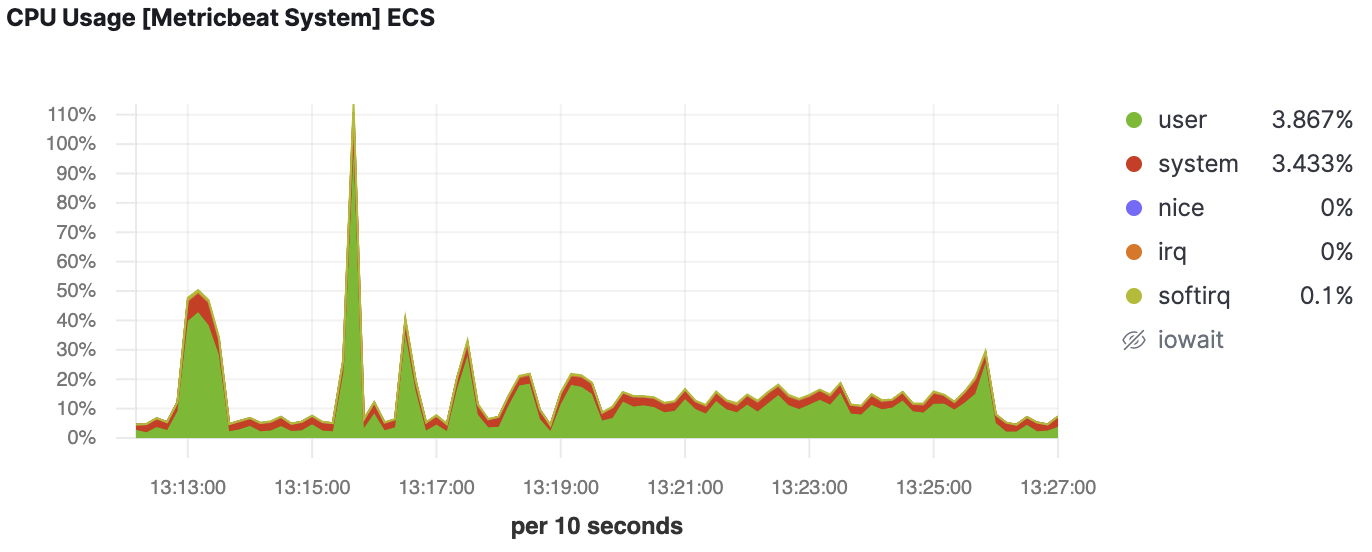
\includegraphics[width=\textwidth]{img/cpu_usage.png}
    \caption{\label{cpu-usage}Zátěž CPU během testu}
\end{figure}

První zvýšení trvající minutu je způsobeno zařízeními ohlašujícími svoje vlastnosti, což způsobilo velký počet zápisů do databáze. Druhé zvýšení ve 13:15:40 trvající 20 vteřin způsobilo přidání jednotlivých zařízení uživatelům (a jejich spárování). Následujících 10\,min trvající zatížení bylo způsobeno tím, že zařízení odesílají data ze svých vlastností. Závěrečná několika vteřinová zvýšená zátěž ve 13:25:50 je dána odesláním informace o odpojení ze všech zařízení. V průběhu testu byla průměrná doba vyřízení databázové operace 0,24 ms, zátěž cpu databází 8 \%, procesem platformy 6 \% a zátěž disku přibližně 2 \%. V průběhu celého testu byla platforma aktivně využívána uživatelem přes webové rozhraní k ovládání fyzických zařízení a po celou dobu vše reagovalo ihned bez jakéhokoliv zpoždění, ani průměrná doba zpracování RESTful požadavku nebyla významně ovlivněna. Z výsledku testu tedy vyplývá, že platforma zvládne bez jakýchkoliv problémů obsloužit stovky zařízení bez negativního dopadu na výkon.


\section{Uživatelské testování}
Za pomoci uživatelského testování byla ověřena intuitivnost uživatelského prostředí. Cílem bylo zjistit, zda uživatelé zvládnou vykonat základní úkony bez pomoci a zjistit jejich náročnost.

Každý uživatel dostal uživatelskou příručku (příloha \ref{user-guide}), přístup k již naprogramovanému zařízení, které ovládalo led světla a měřilo teplotu, a nakonec seznam úkonů, které mají vykonat a zpětně je ohodnotit na stupnici od jedné do pěti (pět je nejhorší). První tester byl muž, věk 49, se zájmem o techniku. Druhý byl také muž, věk 30, s ekonomickým vzděláním.


\begin{figure}
    \centering
    \begin{tabular}{ | l | c | c | }
        \hline
        Úkon                           & Uživatel 1 & Uživatel 2 \\
        \hline
        Připojte nové zařízení         & 4          & 3          \\
        \hline
        Zapněte led světla             & 1          & 1          \\
        \hline
        Podívejte se na průběh teplotu & 2          & 2          \\
        \hline
        Změňte umístění zařízení       & 1          & 1          \\
        \hline
        Zařízení odstraňte             & 1          & 1          \\
        \hline
    \end{tabular}
    \caption{Hodnocení jednotlivých testerů}
\end{figure}

V průběhu testování se ukázal jako nejvíce problematický první krok, ve kterém uživatel zadává v kaptivním portále údaje k připojení na domácí Wifi a své uživatelské jméno k platformě. Zařízení občas ohlásilo chybu připojení k Wifi i při správně zadaných údajích. Ostatní části testu již probíhaly bez jakéhokoliv problému. Dle závěrečného hodnocení se rozhraní ukázalo jako uživatelsky velmi přívětivé a zařízení po úspěšném připojení k Wifi pracovalo již naprosto spolehlivě. Po ukončení testu byly uživatelé v nezávazném rozhovoru dotázáni na možná vylepšení. Z rozhovoru vyplynulo doporučení do budoucna k vytvoření interaktivního průvodce, který by při první návštěvě vysvětlil pokročilejší funkce.

Po bližším zkoumání problematického připojení byl zjišten problém s knihovnou \textit{WifiManager}, která má na starosti vytvoření kaptivního portálu a následné připojení na Wifi. Aktuální verze této knihovny prochází rapidním vývojem s nedostatečnou dokumentací aktuálních funkcí. Nepodařilo se identifikovat, zda je problém se špatným využitím této knihovny či v implementaci knihovny samotné. Pro nalezení řešení bude kontaktován autor knihovny a v případě neúspěchu je možnost využití jiné knihovny implementující podobnou funkcionalitu např. \textit{IotWebConf}.